\documentclass{article}
\title{Physics 5A Homework}
\author{Eric Du}
\date{\today}
\usepackage[cm]{sfmath}
\usepackage{amsmath}
\usepackage{mathtools}
\usepackage{amsfonts}
\usepackage{amssymb}
\usepackage{amsthm}
\setlength{\parindent}{0pt}
\linespread{1.3}
\allowdisplaybreaks
\usepackage{fancyhdr}
\pagestyle{fancy}
\cfoot{\thepage}
\usepackage{float}
\lhead{Eric Du}
\chead{Physics 5A Homework}
\rhead{\today}
\usepackage{epigraph}
\setlength{\epigraphwidth}{148pt}
\usepackage{color}
\renewcommand{\labelitemi}{\textendash}
\renewcommand{\abstractname}{}
\renewcommand{\familydefault}{\sfdefault}
\usepackage[sexy]{evan}
\theoremstyle{definition}
\newtheorem*{solution}{\color{blue}Solution}
\usepackage{caption}
\numberwithin{equation}{section}
\numberwithin{definition}{section}
\begin{document}
	\maketitle
	
	\begin{abstract}
		\noindent \textbf{[NOTE:]} I primarily worked with \textbf{Andrew Binder}, \textbf{Rebecca Feng} and \textbf{Aren Martinian} to complete this assignment.
	\end{abstract}
	\section{Problem 1}
	We have the spacetime invariant for both frames, which allows us to bypass the Minkowski diagram:
	
	\begin{align*}
		s^2 &= (ct)^2-x^2\\
		s'^2 &= (ct')^2 - x'^2
	\end{align*}

	Notice that $x = 0$ in this case since both events are simultaneous, but $x'$, the value we're trying to solve, is nonzero since there is a space separation between these two events. Now we can solve for $x'$, since $s = s'$ from the invariant:
	
	\begin{align*}
		(ct)^2 &= (ct')^2 - x^2\\
		x'^2 &= 36c^2 - 16c^2 = 20c^2\\
		\therefore x &= 2\sqrt{5}c
	\end{align*}

	\section{Problem 2}
	
	We again use the spacetime invariant for this problem: 
	
	\begin{align*}
		(ct)^2 -x^2 &= (ct')^2 - x'^2\\
		-(1)^2 &= (c^2t'^2) -2^2\\
		\therefore t^2 &= \frac{3}{c^2} \implies t' = \frac{\sqrt{3}}{c}
	\end{align*}


	\section{Problem 3}
	Refer to the following diagram:
	
	\begin{figure}[H]
		\centering
		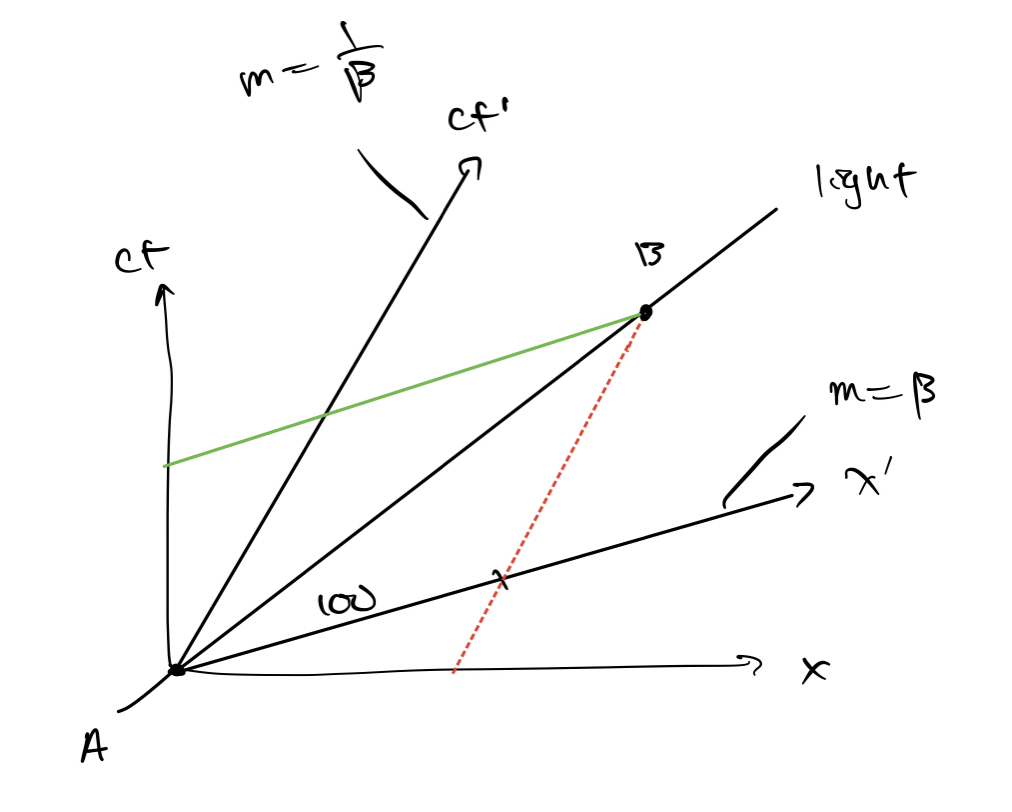
\includegraphics[scale=0.3]{Q3-1.jpg}
		\end{figure}
	
	We have simple length contraction:
	
	\[ L' = \frac{L_0}{\gamma} \implies L' = 80 \ \text{m}\]
	
	This means that we can make the following additions to our diagram:
	
	
	\begin{figure}[H]
		\centering
		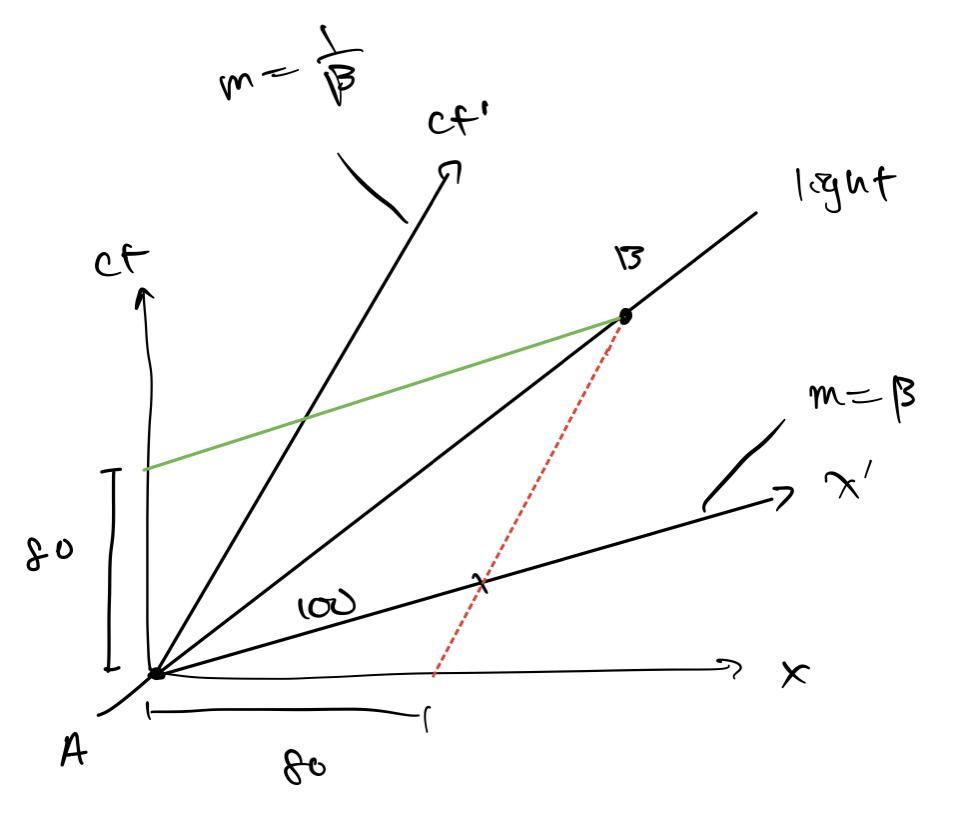
\includegraphics[scale=0.3]{Q3-2.jpg}
		\end{figure}
	
	From here, we can use equations of lines to come up with the following two relationships:
	
	\begin{align*}
		ct &= 0.6x + 80\\
		x &= 80 + 0.6x
	\end{align*}

	Where 0.6 = $\beta$ which was given to us. Now solving these two equations, we get:
	
	\begin{align*}
	x &= 200\\
	t &= \frac{200}{c}
	\end{align*}

	\section{Problem 4}
	
	We can use the velocity transform to find the answer here:
	
	\[ v' = \frac{u-v}{1-\frac{uv}{c^2}}\]
	
	Where $u$ and $v$ are measured from a stationary frame. Thus, we have:
	
	\begin{align*}
		v' &= \frac{0.99c - (-0.99c)}{1+0.99(0.99)}\\
		&= 0.99995c
	\end{align*}

	
	\section{Problem 5}
	
	\subsection{Part a}
	
	Refer to the following diagram:
	
	
	\begin{figure}[H]
		\centering
		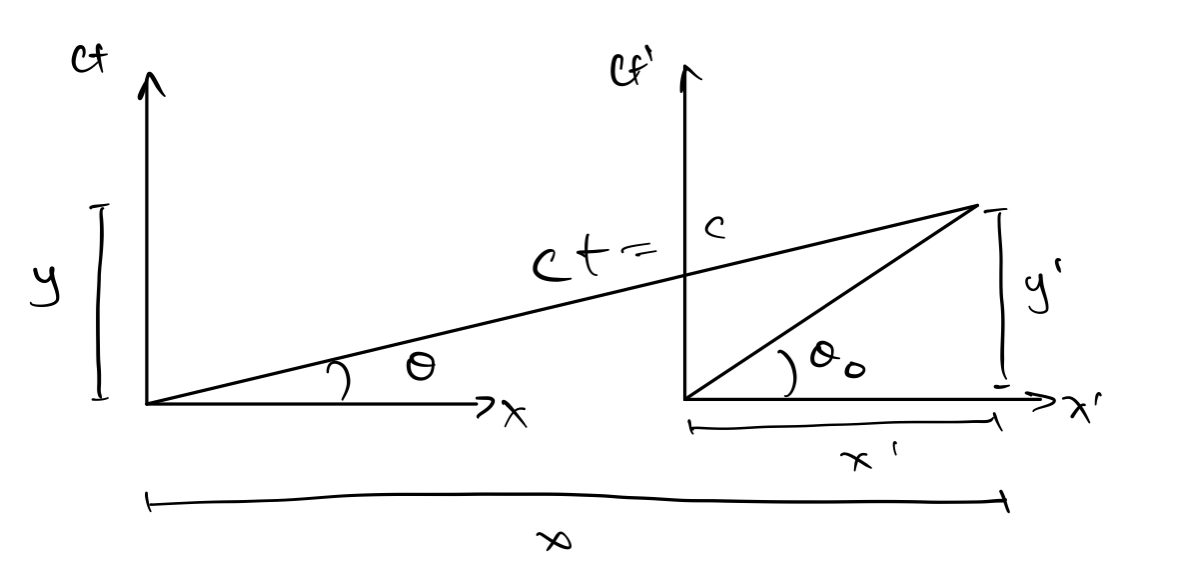
\includegraphics[scale=0.3]{Q5.jpg}
		\end{figure}
	
	We can let the light travel for one second, since that gives us some nice values to work with. We have the relationship $\cos \theta = \frac{x}{ct}$ from simple geometry, and we also have the two lorentz transform equations for $x$ and $t$:
	
	\begin{align*}
		x &= \gamma(x' + vt')\\
		t &= \gamma\left(t' + \frac{v}{c^2}x'\right)
	\end{align*}
	
	If we substitute $t' = 1$ in this case for one second, then we get: 
	
	\begin{align*}
		x &= \gamma(c \cos \theta_0 + v)\\
		t &= \gamma\left(1 + \frac{v}{c} \cos \theta_0\right)
	\end{align*}

	And since we have $\cos \theta = \frac{x}{ct}$, then we can plug $x$ and $t$ into this equation. We get:
	
	\begin{align*}
		\cos \theta &= \frac{\gamma(c \cos \theta_0 + v)}{c\gamma \left(1 + \frac{v}{c} \cos \theta_0\right)}\\
		\therefore \theta &= \cos^{-1}\left(\frac{c \cos \theta_0 + v}{c(1 + \frac{v}{c} \cos \theta_0)}\right)
	\end{align*}
	
	\subsection{Part b}
	
	We have $v_x = \dfrac{x}{t} = c \cos \theta$, where $\theta$ is the angle ($10^{-3}$) radians. (this is true simply because we've allowed the source to radiate light for only one second, so $ct = c$ in this case). Doing so gives us that the velocity of this source is 0.999999945169c.
	
	\section{Problem 6}
	
	\subsection{Parts a, b, c}
	
	Refer to the following diagram for the answers to these parts. They're all diagram drawing, so I've combined all of them into one single diagram: 
	
	\begin{figure}[H]
		\centering
		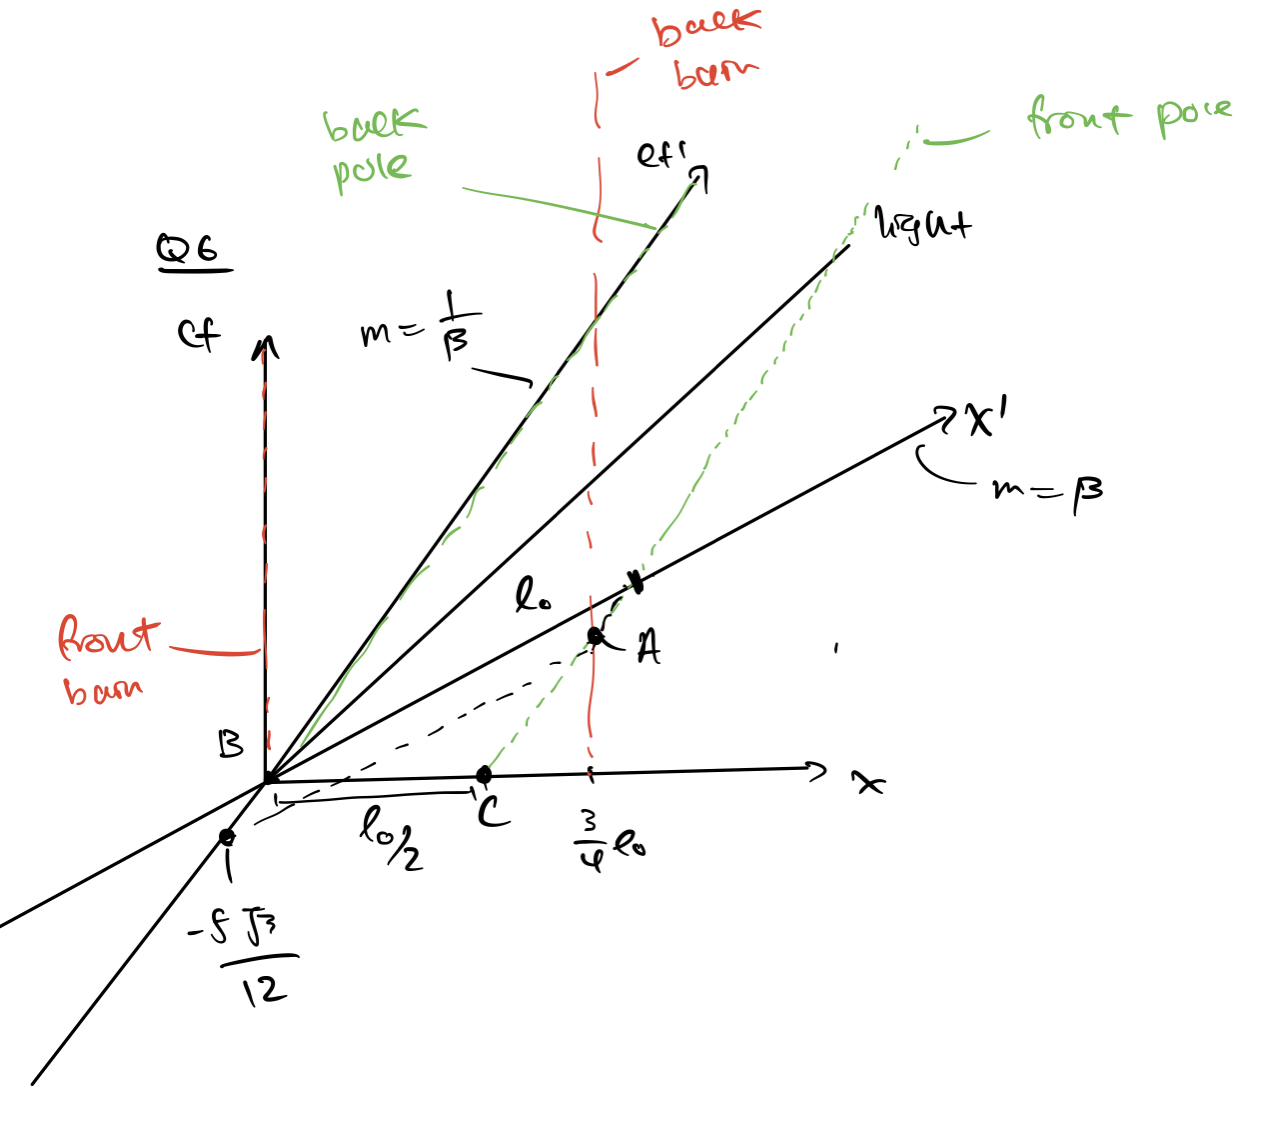
\includegraphics[scale=0.3]{Q6.jpg}
	\end{figure}
	\subsection{Part d}
	
	From the farmer's point of view, we have:
	\[x' = \gamma (x - vt)\]
	
	Since the measuring time is instantaneous (according to the question), the latter term drops to zero. Thus, we have:
	
	\[ x = \frac{x'}{\gamma} \implies l = \frac{l_0}{2}\]
	
	Thus, the pole fits inside the barn completely. This means that the front of the pole is inside the barn when B occurs.
	
	\subsection{Part e}
	For this problem, I solved it using equations of lines. We have the point $(\dfrac{l_0}{2}, 0)$ as a point on the $x$ axis in the $S$ frame. Also, we know that the world line for the front of the pole has slope equivalent ot the $ct'$ axis, which is $\dfrac{1}{\beta}$. Knowing all this, we can plug this into the point slope form for the equation of a line:
		
		\begin{align*}
			y - 0 &= \frac{1}{\beta}\left(x - \frac{l_0}{2}\right)\\
			y &= \frac{2}{\sqrt{3}}x - \frac{l_0}{\sqrt{3}}
		\end{align*}
	
	Now that we have the equation of a line, we can substitute $x = \dfrac{3}{4}l_0$ to find the $y$-coordinate of $A$:
	
	\begin{align*}
		y_A &= \frac{2}{\sqrt{3}}\left(\frac{3}{4}l_0\right) - \frac{l_0}{3}\\
		&= l_0\left(\frac{\sqrt{3}}{2} - \frac{1}{\sqrt{3}}\right)\\
		&= \frac{\sqrt{3}}{6} l_0
		\end{align*}
	
	Thus the coordinates of $A$ in the farmer's frame is $\left(\dfrac{3}{4}l_0, \dfrac{\sqrt{3}}{6}l_0\right)$. This implies that $A$ occurs before $B$ from his perspective.
	
	\subsection{Part f}

We again have a matrix with a lorentz transform, except time it's slightly more annoying:

\[ A' = \begin{bmatrix}
	x_A' \\
	t_A' 
\end{bmatrix} = \begin{bmatrix}
\gamma(x - \frac{v}{c} \cdot ct) \\
\gamma \left(t - \frac{vx}{c^2}\right) 
\end{bmatrix}\]

This means that we have the following to solve:

\begin{align*}
	x_A'= \gamma\left(x - \frac{v}{c} \cdot ct\right) &= 2\left(x - \frac{\sqrt{3}}{2} \cdot \frac{\sqrt{3}}{6}l_0\right) \\
	&= 2\left(\frac{3}{4}l_0 - \frac{3}{12}l_0\right)\\
	&= 2\left(\frac{6}{12} l_0\right) = l_0
\end{align*}

Similarly,

\begin{align*}
	t_A' = \gamma\left(t - \frac{vx}{c^2}\right) &= \gamma(ct - \beta x)\\
	&= 2\left(\frac{\sqrt{3}}{6}l_0 - \frac{3 \sqrt{3}}{8}l_0\right)\\
	&= -\frac{5\sqrt{3}}{12}l_0
\end{align*}
Thus the coordinates of $A$ in the vaulter's frame is $\left(l_0, \dfrac{-5\sqrt{3}}{12}l_0\right)$. This implies that $A$ occurs after $B$ from his perspective.

\subsection{Part g}

Since the barn is length contracted, the rear of the pole is \textbf{not} inside the barn when event $A$ occurs. This can be seen since $A$ occurs after $B$ from the diagram, in other words the front of the pole has already left the barn before the back has had time to go through the barn. This can also be explained if we imagine a pole going through a barn which is clearly too short to fully fit the pole within it.

\subsection{Part h}

Since both reference frames are equally correct, the answer is that both the farmer and the vaulter win the bet, or none of them win at all. This is because there is no ``objective" reference frames, so what both the vaulter and the farmer perceive, as different as they are, are both correct within their reference frames.

\section{Problem 7}

We have the formula for relativistic kinetic energy to be $KE = (\gamma -1)m_0c^2$, whereas we have $\frac{1}{2} mv^2$ classically. If we want to find the fractional error between the two kinetic energies, we have: 

\begin{align*}
	\text{fractional error} &= \frac{E_r - E_c}{E_r}\\
	&= \frac{m_0c^2(\gamma-1) - \frac{1}{2}mv^2}{m_0c^2(\gamma-1)}\\
	&= 1 - \frac{v^2}{2c^2(\gamma-1)}
\end{align*}
	
	If we substitute in the values for velocity for parts a), b), and c), we get a fractional error of $8.33 \times 10^{-10}$, 0.0075062 and 0.68705 respectively.
	
	
	\section{Problem 8}
	
	We have the equation $E^2 = (mc^2)^2 + (pc)^2$. Since we assume the object to not be moving, then we have the latter term equal to zero, so $E = mc^2$. This means that $m = \frac{E}{c^2}$, or approximately 888.8 kilograms.
	
	\section{Problem 9}
	
	The energy released is 484 kJ. If we do the same as problem 8, then we get that a mass of approximately $5.38 \times 10^{-12}$ kilograms has been converted into energy. The total mass of the system is two moles of hydrogen (having molar mass 1.01g/mol) and one mole of oxygen (having molar mass 16.00 g/mol). Since hydrogen and oxygen are diatomic, this means that the total mass has to be multiplied by 2, giving us 36.04g of atoms. Thus, the fraction of that which is converted into energy is:
	
	\[\frac{5.38\times 10^{-9} \ \text{g}}{36.04 \ \text g} = \boxed{1.492\times 10^{-10}}\]
	
	\section{Problem 10} 
	\subsection{Part a} 
	The total energy of the particle is going to be $\gamma m_0c^2$. This means that $\gamma = \frac{E}{m_0c^2}$. We also have that $10^{20}$ eV is approximately 16.02 Joules. This gives us a $\gamma$ value of $1.065 \times 10^{11}$.
	
	\medskip
	
	The proper time in the proton's frame is $t = \dfrac{d'}{v}$, where $d'$ is the perceived length of the galaxy from the proton's point of view. This means that we can write $t = \dfrac{d_0}{\gamma v}$, where $d_0$ is the length of the galaxy from our point of view. 
	
	\medskip
	
	We have the energy of the proton to be equivalen to $E = \gamma m_pc^2$. From here, there are two routes we can take to solve this problem. The first is to approximate the velocity of the proton as $c$ since the energy is so high, in which means that we have the following:
	
	\begin{align*}
		t &= \frac{d_0}{\gamma c}\\
		&= \frac{d_0}{\frac{E}{m_pc^2} c}
	\end{align*}

	This gives us a proper time of $\boxed{29.58}$ seconds. Secondly, since a photon travels at light speed, then time is infinitely dilated, meaning that the proper time for the proton is 0 seconds.
	
	
	\subsubsection{Alternative Method}
	
	Alternatively, we could also not approximate for $v$ and we can solve for $v$ instead, by substituting our $\gamma(v)$ properly. Doing so gives us the following relationship for v:
	
	\[ v= c\sqrt{1 - \frac{m_p^2c^2}{E^2}}\]
	
	Which when we substitute back into our equation for proper time, we get:
	
	\[t = \frac{m_pd_0}{E} \cdot \frac{1}{\sqrt{1- \frac{m_p^2c^2}{E^2}}}\]
	
	Substituting all the values, we get $\boxed{29.58}$ as well. This just goes to show how close to the speed of light these particles are travelling, since we are getting the same values even with an approximation that the velocity of the proton is \textit{equal} to the speed of light, despite that being impossible.
	
	\subsection{Part b}
	
	The energy of a baseball can be calculated as $\dfrac{1}{2}mv^2$, which 144.88 Joules, whereas the energy of the proton is $10^{20}$ electronvolts, which changes to 16.02 Joules. By comparison this seems small, but we have to remember that a proton has a very small mass, so this is actually a very large amount of energy.
	
	\section{Problem 11}
	
	We have the velocity transform:
	
	\[v' = \frac{u-v}{1+ \frac{uv}{c^2}}\]
	
	Thus we can put our velocities in, and since they're the same for both particles, then we get:
	
	\[ v' = \frac{v - (-v)}{1 + \frac{v^2}{c^2}} = \frac{2v}{1 + \frac{v^2}{c^2}}\]
	
	To make the next few calculations simpler, we're going to rearrange the above formula to:
	
	\[ v' = \frac{2vc^2}{c^2 + v^2}\]
	
	We can now calculate $\gamma$:
	
	\begin{align*}
		\gamma &= \frac{1}{\sqrt{1 - \frac{v'^2}{c^2}}}\\
		&= \frac{1}{\sqrt{1-\frac{(2vc^2)^2}{(c^2 + v^2)c^2}}}\\
		&= \frac{1}{\sqrt{1-\frac{4v^2c^2}{(c^2 + v^2)^2}}}\\
		&= \frac{1}{\sqrt{\frac{(c^2 + v^2)^2 - 4c^2v^2}{(c^2 + v^2)^2}}}\\
		&= \frac{1}{\sqrt{\frac{c^4 - 2c^2v^2 + v^4}{(c^2 +v^2)^2}}}\\
		&= \frac{1}{\sqrt{\frac{(c-v)^2}{(c+v)^2}}}\\
		&= \frac{c+v}{c-v}
	\end{align*}

	Thus, we have:
	
	\[ E = \frac{c+v}{c-v}m_0c^2\]


	\section{Problem 12}
	
	The momentum is conserved in this case, and although the mechanical energy is not conserved, the total energy remains conserved. Thus we can write the following two conservation formulas:
	
	\begin{align*}
		\gamma_im_0v &= \gamma_f(m_0 + M)v'\\
		\gamma_im_0c^2 + Mc^2 &= \gamma_f (m_0 + M)c^2
	\end{align*}

	The easiest way to solve this system of equations is if we just divide both equations, cancelling the $\gamma_f$ term entirely. Thus, we can solve:
	
	\begin{align*}
		\frac{\gamma_i m_0v}{c^2(\gamma_im_0 + M)} &= \frac{v'}{c^2}\\
		\therefore \frac{\gamma_i m_0v}{\gamma_im_0 + M} = v' 
	\end{align*}


	\section{Problem 13}
	
	We can write the initial and final four-momentums for both particles:
	
	\begin{align*}
		\text{photon (initial)}& P_{\varepsilon i} = \left(\frac{\varepsilon_i}{c}, \frac{\varepsilon_i}{c}, 0, 0\right)\\
		\text{electron (initial)}& P_{ei} = (m_0c, 0, 0, 0)\\
		\text{photon (final)}& P_{\varepsilon f} = \left(\frac{\varepsilon_f}{c}, \frac{\varepsilon}{c}\cos\theta, \frac{\varepsilon}{c} \sin\theta, 0\right)\\
		\text{electron (final)}& P_{ef} = (m_0c, p_f \cos \varphi, p_f\sin\varphi, 0)
	\end{align*}

	We have conservation of momentum in the $x$ and $y$ directions, meaning we take the second and third index of the initial and final four momenta matrices respectively:
	
	\begin{align*}
		\frac{\varepsilon_i}{c} &= p_f \cos \varphi  + \frac{\varepsilon_f}{c} \cos \theta\\
		0 &= \frac{\varepsilon_f}{c}\sin \theta - p_f \sin \varphi
		\end{align*}
	
	Rearranging this we get:
	
	\begin{align*}
		p_f \cos \varphi &= \frac{\varepsilon_i}{c} - \frac{\varepsilon_f}{c}\cos\theta\\
		p_f \sin \varphi &= \frac{\varepsilon_f}{c}\sin \theta
	\end{align*}

	Again, just like the last problem, we can divide the top equation by the bottom one, getting us:
	
	\begin{equation}\label{q13}
		cot \varphi = \frac{\epsilon_i}{\epsilon_f} \cdot \frac{1}{\sin \theta} - \cot \theta
		\end{equation}
	
	So we also have the following equation, which can be found as a result in example 13.6 in the textbook showcasing Compton scattering:
	
	\[\varepsilon_f = \frac{\varepsilon_i}{1 + \frac{\varepsilon_i}{m_0c^2}(1-\cos \theta)}\]
	
	This equation comes from the conservation of energy and was also discussed in Emil's final review as a standalone problem. The derivation for this formula alone was presented as a standalone problem, so I won't write out the full derivation here. We can also rearrange this formula to make it a bit nicer to work with:
	
	\[ \varepsilon_f = \frac{m_0c^2\sin\theta}{m_0c^2 + \varepsilon_i(1-\cos\theta)}\]
	
	Now we can substitute this formula for $\varepsilon_f$ into equation \ref{q13} and we get: 
	
	\begin{align*}
		\cot \varphi &= \frac{\varepsilon_i (m_0c^2 + \varepsilon_i(1-\cos \theta))}{\varepsilon_i m_0c^2 \sin \theta} - \cot \theta\\
		&= \frac{1}{\sin \theta} - \cot \theta + \frac{\varepsilon_i (1-\cos \theta)}{m_0c^2 \sin \theta}\\
		&= \left(1 + \frac{\varepsilon_i}{m_0c^2}\right)\tan\left(\frac{\theta}{2}\right)
		\end{align*}
	
	
	\section{Dango}
	
	We have $P(x) + P(-x) = P(0)$ for all real $x$ so $P(0) + P(0) = P(0) \implies P(0) = 0$. We also know that since this is true, then $P(x)$ must be a polynomial of odd degree. Now we compute $P(1)$ and $P(-1)$:
	
	\begin{align*}
		P(1) &= \sum_n a_n\\
		P(-1) &= \sum_n (-1)^na_n
	\end{align*}

	Notice that when we add $P(1) + P(-1)$ all the terms with even $x$ exponents don't cancel. Thus for the condition to be true ($P(1) + P(-1) = 0$), then we require that $P(x)$ has no terms with even exponents of $x$. 
	
	\medskip
	
	Now if we write $P(x) = x^{2m+1} + x^{2n-1}$ then we can always common factor the lower exponent and the remaining as a difference of exponents, which always gives us a root. If we have another root, then symmetry is broken since it means that for some nonzero $x$, $P(x) = 0$, which won't satisfy $P(x) + P(-x) = 0$ (this is obviously true since $P(x)$ is odd, and $P(-x)$ can never be zero if $P(x) = 0$)
	
	\medskip
	
	Otherwise, if we write $P(x) = x^{2m+1} - x^{2n-1}$, then notice that for $P(1) = 1$ then we have to write $P(x) = \frac 1 k (x^{2n+1} + \dots)$, where $k$ denotes the number of terms in $P(x)$. This means we get $P(-1) = \frac{-k}{k} = -1$ , meaning that $P(-1) = -1$ is the only solution.
	
	
	$$ f(x) = kx$$
	\[f(x) = kx\]
	
\end{document}